\documentclass{standalone}
\usepackage{tikz}
\usetikzlibrary{
  shapes.geometric, 
  positioning, 
  backgrounds
}

\usepackage{xcolor}
\definecolor{mybgcolor}{HTML}{F8F9FA}

\begin{document}

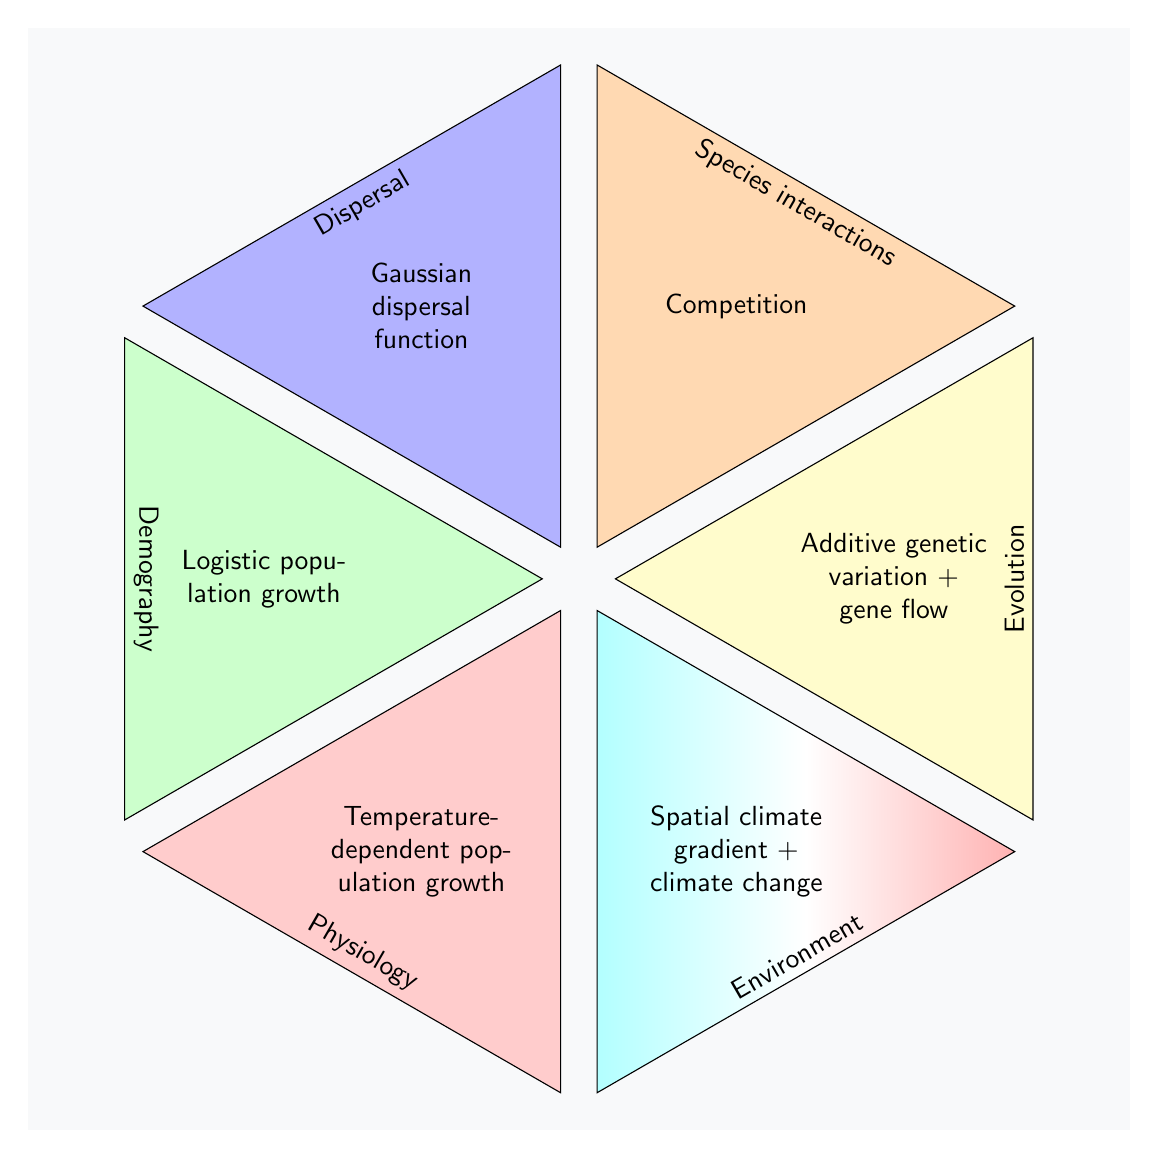
\begin{tikzpicture}[
  my_triangle/.style={
    draw,
    regular polygon,
    regular polygon sides=3,
    minimum size=3.5cm,
    inner sep=0pt,
    text width=2.5cm,
    align=center,
    font=\sffamily,
  }
  ]

  \path[use as bounding box] (-7,-7) rectangle (7,7);

  \begin{scope}[on background layer]
    \fill[mybgcolor] (current bounding box.south west) rectangle (current bounding box.north east);
  \end{scope}

  \node[my_triangle, fill=yellow!20, shape border rotate=90] (evolution) at (0:4cm) {Additive genetic variation + gene flow};
  \path (evolution.corner 2) -- node[midway, sloped, above, font=\sffamily] {Evolution} (evolution.corner 3);

  \node[my_triangle, fill=orange!30, shape border rotate=150] (competition) at (60:4cm) {Competition};
  \path (competition.corner 2) -- node[midway, sloped, below, font=\sffamily] {Species interactions} (competition.corner 3);

  \node[my_triangle, fill=blue!30, shape border rotate=-150] (dispersal) at (120:4cm) {Gaussian dispersal function};
  \path (dispersal.corner 2) -- node[midway, sloped, below, font=\sffamily] {Dispersal} (dispersal.corner 3);

  \node[my_triangle, fill=green!20, shape border rotate=-90] (demography) at (180:4cm) {Logistic population growth};
  \path (demography.corner 2) -- node[midway, sloped, above, font=\sffamily] {Demography} (demography.corner 3);
  
  \node[my_triangle, fill=red!20, shape border rotate=-30] (physiology) at (240:4cm) {Temperature-dependent population growth};
  \path (physiology.corner 2) -- node[midway, sloped, above, font=\sffamily] {Physiology} (physiology.corner 3);

  \node[my_triangle, left color=cyan!30, right color=red!30, middle color=white, shape border rotate=30] (environment) at (300:4cm) {Spatial climate gradient + climate change};
  \path (environment.corner 2) -- node[midway, sloped, above, font=\sffamily] {Environment} (environment.corner 3);

\end{tikzpicture}

\end{document}
